% Quick start guide
\documentclass{beamer}

% \usepackage[colorlinks=true]{hyperref}
\usepackage{hyperref}
\usepackage{natbib}
\usepackage{apalike}
\usepackage{amsthm}

\usetheme{default}

\newtheorem{probDef}{Definition}
\newtheorem*{probDef*}{Definition}
\newtheorem{claim}{Claim}
\newtheorem*{claim*}{Claim}
\newtheorem*{lemma*}{Lemma}
\newtheorem{probExample}{Example}
\newtheorem{probRule}{Rule}
\newtheorem{probAxiom}{Axiom}
\setbeamertemplate{theorems}[numbered]
\newtheorem{probExercise}{Exercise}

\newtheorem{manualprobRuleinner}{Rule}
\newenvironment{manualProbRule}[1]{%
  \renewcommand\themanualprobRuleinner{#1}%
  \manualprobRuleinner
}{\endmanualprobRuleinner}

\newtheorem{manualprobExampleinner}{Example}
\newenvironment{manualProbExample}[1]{%
  \renewcommand\themanualprobExampleinner{#1}%
  \manualprobExampleinner
}{\endmanualprobExampleinner}

\newcounter{saveenumi}
\newcommand{\seti}{\setcounter{saveenumi}{\value{enumi}}}
\newcommand{\conti}{\setcounter{enumi}{\value{saveenumi}}}
\newcommand{\keepi}{\addtocounter{saveenumi}{-1}\setcounter{enumi}{\value{saveenumi}}}

\DeclareMathOperator*{\argmax}{arg\,max}
\DeclareMathOperator*{\argmin}{arg\,min}

% Title page details
\title{Bonsai.ML}
\subtitle{Intelligent Experimental Control}
\author{Nicholas Guilbeault and Gon\c{c}alo Lopes and Joaqu\'{i}n Rapela}
\institute{Gatsby Computational Neuroscience Unit\\NeuroGEARS Ltd.}
\date{December 5, 2024}

\AtBeginSection[ ]
{
\begin{frame}{Outline}
    \tableofcontents[currentsection]
\end{frame}
}

\begin{document}

\begin{frame}
	\titlepage
\end{frame}

\begin{frame}{Outline}
    \tableofcontents
\end{frame}

\section{Introduction}

\begin{frame}
    \frametitle{History of Bonsai.ML}

    \begin{itemize}

        \item grant application

        \item developing tools

        \item who cares about Bonsai.ML tools? $\rightarrow$ more focus on
            dissemination

        \item real-time ML

    \end{itemize}
\end{frame}

\begin{frame}
    \frametitle{Goals of Bonsai.ML}

    \begin{itemize}
        \item allow non-programmers use ML tools,
        \item learn from non-programmers what ML tools are useful for them
    \end{itemize}
\end{frame}

\begin{frame}
    \frametitle{Need for Real-Time and Reactive ML}

    Conventional ML operates on stored datasets. We need real-time ML that
    operates on infinite data stream with time-varying statistical properties.

    If a sensor fails, our inferences need to continue. That is, we need
    reactive ML (e.g., \href{https://rxinfer.ml/}{rx.infer}).
\end{frame}

\begin{frame}
    \frametitle{Bonsai.ML demos}

\end{frame}

\section{Linear Regression}

\begin{frame}
    \frametitle{Linear Regression: Fundamental Concepts}

    \begin{itemize}
        \item main concepts of linear regression
        \item Online Bayesian Linear Regression (can process infinite data streams, but assumes stationarity)
        \item Recursive least squares (can process infinite data streams, and
            does not assume stationarity)
    \end{itemize}

\end{frame}

\begin{frame}
    \frametitle{Linear Regression: Practical}

    Estimation of receptive fields of visual cells from the Allen Institute.

\end{frame}

\begin{frame}
    \frametitle{Linear regression example}

	\begin{center}
		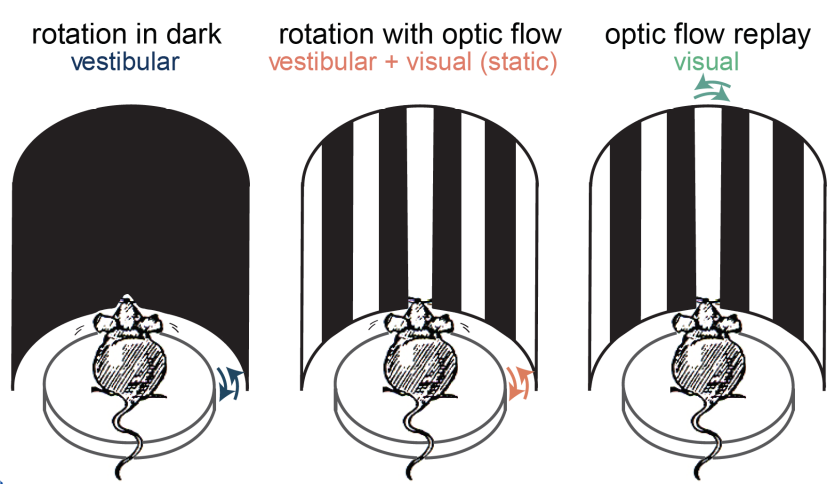
\includegraphics[width=2.2in]{figures/visVesIntegration.png}
	\end{center}
	\hfill\href{https://www.biorxiv.org/content/10.1101/2021.01.22.427789v4.abstract}{Keshavarzi et al., 2021}
	\begin{columns}
		\onslide<2->{
		\begin{column}{0.5\textwidth}
			\begin{center}
				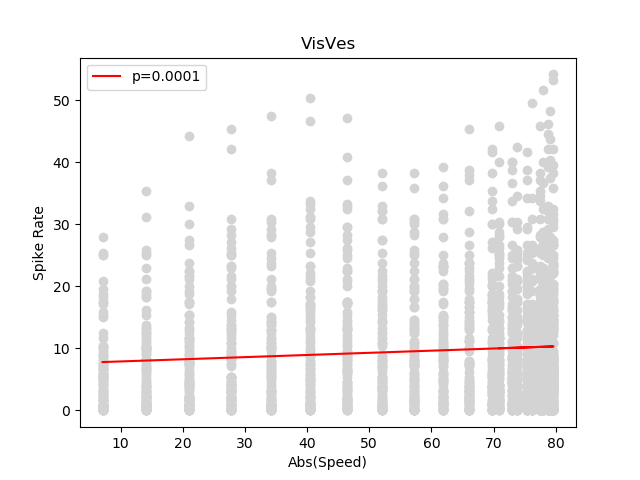
\includegraphics[width=1.5in]{figures/spikeRateVsabsSpeedV1VisVes.png}
			\end{center}
		\end{column}
		}
		\onslide<3->{
		\begin{column}{0.5\textwidth}
			\textcolor{blue}{Is there a linear relation between the speed of rotation and the firing rate of visual cells?}
		\end{column}
		}
	\end{columns}
\end{frame}

\begin{frame}
    \frametitle{Estimating nonlinear receptive fields from natural images}

    \tiny
    \begin{eqnarray}
        y(\mathbf{x})&=&k_{0}+\sum_{i,j=1}^{N}k_{1}(i, j)x(i, j)\label{eq:volterraSpatial}\\
        &+&\sum_{i_{1},j_{1},i_{2},j_{2}=1}^{N}k_{2}(i_{1},j_{1},i_{2},j_{2})x(i_{1},j_{1})x(i_{2},j_{2})+\ldots\nonumber\\
        &+&\sum_{i_{1},j_{1},\ldots,i_{Q},j_{Q}=1}^{N}k_{Q}(i_{1},j_{1},\ldots,i_{Q},j_{Q})x(i_{1},j_{1})\ldots
        x(i_{Q},j_{Q})+\;\varepsilon\nonumber\\
        y(\mathbf{x})&=&\mathbf{Aq(x)}+\;\varepsilon
    \end{eqnarray}

		\begin{center}
			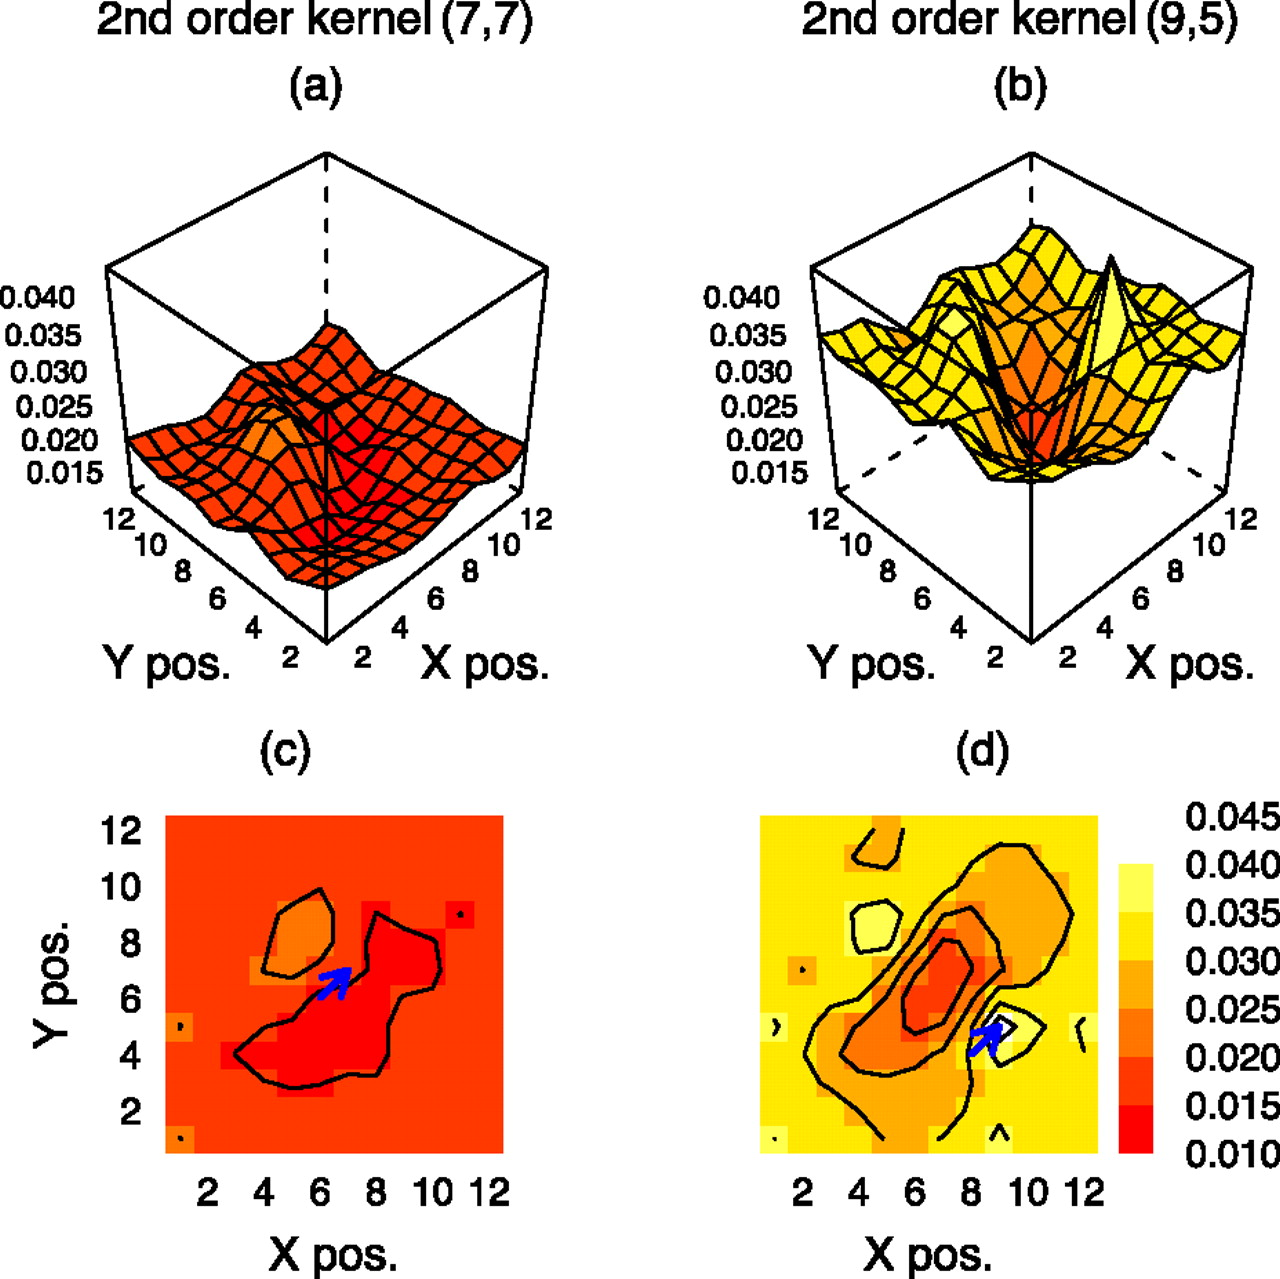
\includegraphics[width=1.5in]{figures/jov-6-4-11-fig020.png}
		\end{center}
        \hfill\scriptsize\href{https://jov.arvojournals.org/article.aspx?articleid=2192869}{Rapela et al., 2006}.

\end{frame}

\begin{frame}
    \frametitle{Linear regression model}

	\scriptsize
	\begin{description}
		\item[simple linear regression model]
			\begin{align*}
                y(x_i, \mathbf{w})&=w_0+w_1x_i
				                   =\raisebox{0.60em}{$[1,x_i]$}
									\left[\begin{array}{c}
								        w_0\\
								        w_1
								    \end{array}\right]
				                   =\raisebox{0.60em}{$[\phi_0(x_i),\phi_1(x_i)]$}
									\left[\begin{array}{c}
								        w_0\\
								        w_1
								    \end{array}\right]\\
                                  & =
									\boldsymbol{\phi}(x_i)^\intercal\mathbf{w}
			\end{align*}
		\item[polynomial regression model]
			\begin{align*}
				y(x_i, \mathbf{w})&=w_0+w_1x_i+w_2x_i^2+w_3x_i^3
				                   =\raisebox{1.80em}{$[1,x_i,x_i^2,x_i^3]$}
									\left[\begin{array}{c}
								        w_0\\
								        w_1\\
								        w_2\\
								        w_3
								    \end{array}\right]\\
				                  &=\raisebox{1.80em}{$[\phi_0(x_i),\phi_1(x_i),\phi_2(x_i),\phi_3(x_i)]$}
									\left[\begin{array}{c}
								        w_0\\
								        w_1\\
								        w_2\\
								        w_3
								    \end{array}\right]=
									\boldsymbol{\phi}(x_i)^\intercal\mathbf{w}
			\end{align*}
		\item[basis functions linear regression model]
			\begin{align*}
				y(x_i, \mathbf{w})&=\boldsymbol{\phi}(x_i)^\intercal\mathbf{w}=\sum_{j=1}^Mw_j\phi_j(x_i)
			\end{align*}
	\end{description}
	\normalsize
\end{frame}

\begin{frame}
    \frametitle{Linear regression model}

    \scriptsize
    \begin{align*}
        \mathbf{y}(\mathbf{x},\mathbf{w})&=
            \left[\begin{array}{c}
                      y(x_1,\mathbf{w})\\
                      y(x_2,\mathbf{w})\\
                      \ldots\\
                      y(x_N,\mathbf{w})
                  \end{array}\right]=
            \left[\begin{array}{cccc}
                      \phi_1(x_1)&\phi_2(x_1)&\ldots&\phi_M(x_1)\\
                      \phi_1(x_2)&\phi_2(x_2)&\ldots&\phi_M(x_2)\\
                      \vdots     &\vdots     &\ldots&\vdots\\
                      \phi_1(x_N)&\phi_2(x_N)&\ldots&\phi_M(x_N)
            \end{array}\right]\left[\begin{array}{c}
                                        w_1\\
                                        w_2\\
                                        \vdots\\
                                        w_M
                                    \end{array}\right]\\
                                         &=\boldsymbol{\Phi}\mathbf{w}
    \end{align*}

    where
    $\mathbf{y}(\mathbf{x},\mathbf{w})\in\mathbb{R}^N,\boldsymbol{\Phi}\in\mathbb{R}^{N\times M},\mathbf{w}\in\mathbb{R}^M$.
    \normalsize
\end{frame}

\begin{comment}

\begin{frame}
    \frametitle{Basis functions for regression}

		\begin{center}
			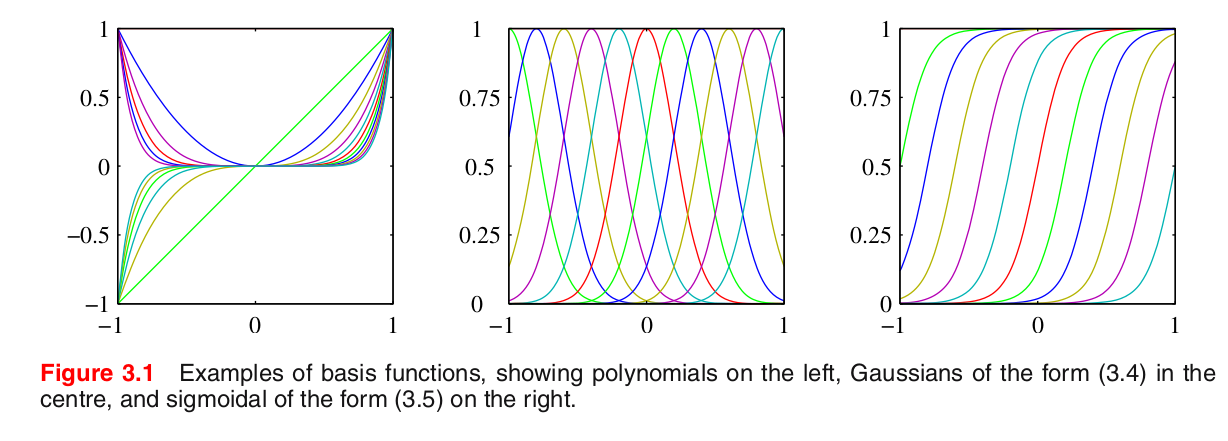
\includegraphics[width=3.5in]{figures/basisFunctions.png}
		\end{center}
        \hfill\scriptsize\citet{bishop06}

        \begin{description}
            \item[polynomial] $\phi_i(x)=x^i$
            \item[Gaussian] $\phi_i(x)=\exp(-\frac{(x-\mu_i)^2}{2\sigma^2})$
            \item[sigmoidal]
                $\phi_i(x)=\frac{1}{1+\exp(-\frac{x-\mu_i}{\sigma^2})}$
        \end{description}
\end{frame}

\begin{frame}
    \frametitle{Example dataset}

    \begin{center}
        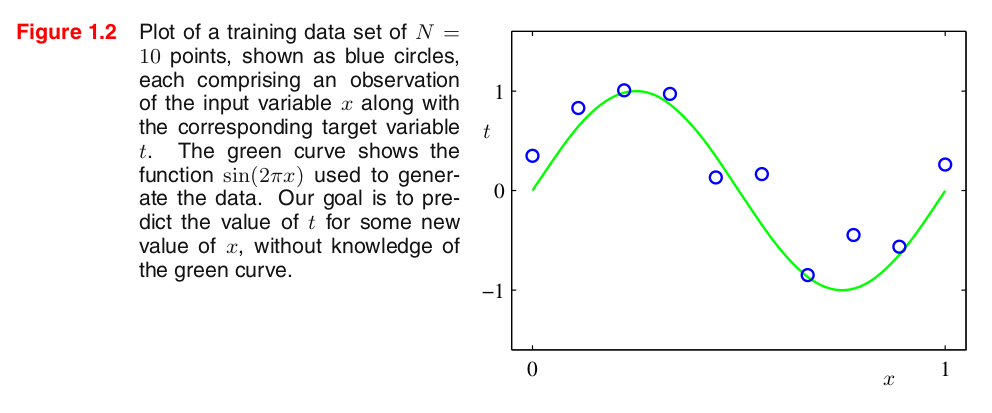
\includegraphics[width=4in]{figures/exampleDataset.png}
    \end{center}
    \hfill\scriptsize\citet{bishop06}

\end{frame}

\end{comment}

\begin{frame}

\begin{alertblock}{Notes}
    \begin{itemize}
        \item We learned how to build a linear regression model.
        \item But, how can we learn the model parameters $w$?
    \end{itemize}
\end{alertblock}

\end{frame}

\subsection{Least-squares regression}

\begin{frame}
    \frametitle{Least-squares estimation of model parameters
    \citep{trefethenAndBau97}}

    \scriptsize
    \begin{probDef}[Least-squares problem]
        Given $\boldsymbol{\Phi}\in\mathbb{R}^{N\times M},N\ge
        M,\mathbf{t}\in\mathbb{R}^N$, find $\mathbf{w}\in\mathbb{R}^M$ such
        that $E_{LS}(\mathbf{w})=||\mathbf{t}-\boldsymbol{\Phi}\boldsymbol{w}||_2$ is minimised.
    \end{probDef}
    \begin{theorem}[Least-squares solution]
        Let $\boldsymbol{\Phi}\in\mathbb{R}^{N\times M} (N\ge M)$ and
        $\mathbf{t}\in\mathbb{R}^N$ be given. A vector
        $\mathbf{w}\in\mathbb{R}^M$ minimises
        $||\mathbf{r}||_2=||\mathbf{t}-\boldsymbol{\Phi}\mathbf{w}||_2$, thereby solving the
        least-squares problem, if and only if
        $\mathbf{r}\perp\text{range}(\boldsymbol{\Phi})$, that is,
        $\boldsymbol{\Phi}^\intercal\mathbf{r}=0$,
        or equivalently,
        $\boldsymbol{\Phi}^\intercal\boldsymbol{\Phi}\mathbf{w}=\boldsymbol\Phi^\intercal\mathbf{t}$,
        or again equivalently,
        $P\mathbf{t}=\boldsymbol{\Phi}\mathbf{w}$,
        where $P\in\mathbf{R}^{N\times N}$ is the orthogonal projector onto
        $\text{range}(A)$ (i.e., $P=A\;(A^\intercal A)^{-1}A^\intercal)$.

    \end{theorem}
	\begin{center}
		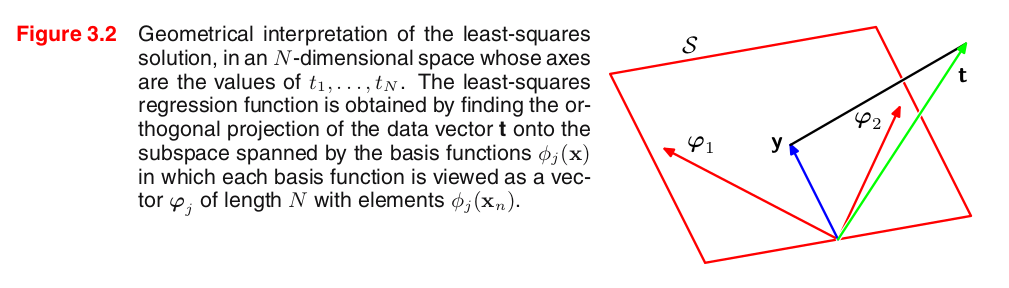
\includegraphics[width=4in]{figures/leastSquares.png}
	\end{center}
    \hfill\scriptsize\citet{bishop06}
    \normalsize

    \note{
    Given a set of $N$ observations, $\mathbf{t}$, $N>M$, we want to find model
    parameters $\mathbf{w}$ such that the model outputs,
    $\mathbf{t}(\mathbf{x},\mathbf{w})$ equal the observations. This is
    generally impossible, because the degrees of freedom of the observations,
    $N$, is generally larger than the degrees of freedom of the model
    $\mathbf{t}(\mathbf{x},\mathbf{w})$, $M$. We instead solve the following
    least-squares problem.
    }
\end{frame}

\begin{frame}[fragile]
    \frametitle{Instruction to run notebooks in Google Colab}

    \begin{enumerate}
        \item open a notebook from
            \href{https://github.com/joacorapela/gcnuBridging2023/tree/master/docs/sphinx/build/html/notebooks/auto_examples/bayesianLinearRegression}{here}
        \item replace \textbf{github.com} by \textbf{githubtocolab.com} in the
            URL
        \item insert a cell at the beginning of the notebook with the following
            content
        \seti
    \end{enumerate}

    \tiny
    \begin{verbatim}
       !git clone https://github.com/joacorapela/gcnuBridging2023.git
       %cd gcnuBridging2023
       !pip install -e .
    \end{verbatim}
    \normalsize

    \begin{enumerate}
        \conti
        \item from the menu \textbf{Runtime} select \textbf{Run all}.
    \end{enumerate}
\end{frame}

\begin{frame}
    \frametitle{Code for least-squares estimation of model parameters}

    \begin{itemize}
        \item \href{https://joacorapela.github.io/gcnuBridging2023/auto\_examples/bayesianLinearRegression/plotOverfittingLeastSquares.html\#sphx-glr-auto-examples-bayesianlinearregression-plotoverfittingleastsquares-py}{overfitting}
        \item \href{https://joacorapela.github.io/gcnuBridging2023/auto\_examples/bayesianLinearRegression/plotCrossValidationLeastSquares.html\#sphx-glr-auto-examples-bayesianlinearregression-plotcrossvalidationleastsquares-py}{cross validation}
        \item \href{https://joacorapela.github.io/gcnuBridging2023/auto\_examples/bayesianLinearRegression/plotLackOfOverfittingInLeastSquaresForLargerDatasetSize.html\#sphx-glr-auto-examples-bayesianlinearregression-plotlackofoverfittinginleastsquaresforlargerdatasetsize-py}{larger datasets allow more complex models}
    \end{itemize}

\end{frame}

\begin{frame}

\begin{alertblock}{Notes}
    \begin{itemize}
        \item We learned how to estimate the parameters of a linear regression
            models by least squares.
        \item But, how to avoid overfitting in the estimation?
    \end{itemize}
\end{alertblock}

\end{frame}

\begin{frame}
    \frametitle{Regularised least-squares estimation of model parameters}

    To cope with the overfitting of least squares, we can add to the least
    squares optimisation criterion a term that enforces coefficients to be
    zero. The regularised least-squares optimisation criterion becomes:

    \begin{align*}
        E_{RLS}(\mathbf{w})=||\mathbf{t}-\boldsymbol{\Phi}\mathbf{w}||_2^2+\lambda||\mathbf{w}||_2^2
    \end{align*}

    where $\lambda$ is the regularisation parameter that weights the strength
    of the regularisation.
\end{frame}

\begin{frame}
    \frametitle{Regularised least-squares estimation of model parameters}
	\scriptsize
	\begin{claim}[Regularised least-squares estimate]
		\begin{align*}
			\mathbf{w}_{RLS}=\argmin_{\mathbf{w}}E_{RLS}(\mathbf{w})=\argmin_{\mathbf{w}}||\mathbf{t}-\boldsymbol{\Phi}\mathbf{w}||_2^2+\lambda||\mathbf{w}||_2^2=(\lambda\mathbf{I}+\boldsymbol{\Phi}^\intercal\boldsymbol{\Phi})^{-1}\boldsymbol{\Phi}^\intercal\mathbf{t}
		\end{align*}
	\end{claim}
	\tiny
	\begin{proof}
		Since $E_{RLS}(\mathbf{w})$ is a polynomial of order two on the elements of $\mathbf{w}$ (i.e., a quadratic form), we can use the \emph{Completing the Squares} technique below to find its minimum.
		\begin{align}
			\boldsymbol{\mu}&=\argmax_{\mathbf{w}}\mathcal{N}(\mathbf{w}|\boldsymbol{\mu},\Sigma)=\argmax_{\mathbf{w}}\log\mathcal{N}(\mathbf{w}|\boldsymbol{\mu},\Sigma)\nonumber\\
                            &=\argmax_{\mathbf{w}}\{K-\frac{1}{2}(-2\boldsymbol{\mu}^\intercal\Sigma^{-1}\mathbf{w}+\mathbf{w}\Sigma^{-1}\mathbf{w})\}\label{eq:completingTheSquaresStep2}\\
                            &=\argmin_{\mathbf{w}}\{-K+\frac{1}{2}(-2\boldsymbol{\mu}^\intercal\Sigma^{-1}\mathbf{w}+\mathbf{w}\Sigma^{-1}\mathbf{w})\}\nonumber\\
                            &=\argmin_{\mathbf{w}}\{K_1-2\boldsymbol{\mu}^\intercal\Sigma^{-1}\mathbf{w}+\mathbf{w}\Sigma^{-1}\mathbf{w}\}\label{eq:completingTheSquares}
		\end{align}

		% Note: Eq.~\ref{eq:completingTheSquaresStep2} uses Eq.~\ref{eq:gaussianQuadratic}.

		To find the minimum of a quadratic form, we write it in the form of the
terms inside the curly brackets of Eq.~\ref{eq:completingTheSquares}, and the
term corresponding to $\boldsymbol{\mu}$ will be the minimum.

		\phantom\qedhere
	\end{proof}
	\normalsize
\end{frame}

\begin{frame}
    \frametitle{Regularised least-squares estimation of model parameters}
	\tiny
		\begin{proof}
			Let's write $E_{RLS}$ in the form of the terms inside the curly brackets of Eq.~\ref{eq:completingTheSquares}.

		\begin{align*}
			E_{RLS}&=||\mathbf{t}-\boldsymbol{\Phi}\mathbf{w}||_2^2+\lambda||\mathbf{w}||_2^2=(\mathbf{t}-\boldsymbol{\Phi}\mathbf{w})^\intercal(\mathbf{t}-\boldsymbol{\Phi}\mathbf{w})+\lambda\mathbf{w}^\intercal\mathbf{w}\\
                   &=\mathbf{t}^\intercal\mathbf{t}-2\mathbf{t}^\intercal\boldsymbol{\Phi}\mathbf{w}+\mathbf{w}^\intercal\boldsymbol{\Phi}^\intercal\boldsymbol{\Phi}\mathbf{w}+\lambda\mathbf{w}^\intercal\mathbf{w}\\
                   &=\mathbf{t}^\intercal\mathbf{t}-2\mathbf{t}^\intercal\boldsymbol{\Phi}\mathbf{w}+\mathbf{w}^\intercal(\boldsymbol{\Phi}^\intercal\boldsymbol{\Phi}+\lambda\mathbf{I}_M)\mathbf{w}
		\end{align*}
		Calling
		\begin{align*}
			\Sigma^{-1}&=\boldsymbol{\Phi}^\intercal\boldsymbol{\Phi}+\lambda\mathbf{I}_M\\
			\boldsymbol{\mu}^\intercal\Sigma^{-1}&=\mathbf{t}^\intercal\boldsymbol{\Phi}\;\text{or}\;\boldsymbol{\mu}^\intercal=\mathbf{t}^\intercal\boldsymbol{\Phi}\Sigma\;\text{or}\;\boldsymbol{\mu}=\Sigma\boldsymbol{\Phi}^\intercal\mathbf{t}=\left(\boldsymbol{\Phi}^\intercal\boldsymbol{\Phi}+\lambda\mathbf{I}_M\right)^{-1}\boldsymbol{\Phi}^\intercal\mathbf{t}
		\end{align*}
		we can express
		\begin{align*}
			E_{RLS}=K+2\boldsymbol{\mu}^\intercal\Sigma^{-1}\mathbf{w}+\mathbf{w}\Sigma^{-1}\mathbf{w}
		\end{align*}
		Then
		\begin{align*}
			 \mathbf{w}_{RLS}=\argmin_{\mathbf{w}}E_{RLS}(\mathbf{w})=\boldsymbol{\mu}=\left(\boldsymbol{\Phi}^\intercal\boldsymbol{\Phi}+\lambda\mathbf{I}_M\right)^{-1}\boldsymbol{\Phi}^\intercal\mathbf{t} 
		\end{align*}
		\end{proof}
	\normalsize
\end{frame}

\begin{frame}
    \frametitle{Code for regularised least-squares estimation of model parameters}
    \begin{itemize}
        \item \href{https://github.com/joacorapela/gcnuBridging2023/blob/master/docs/sphinx/build/html/notebooks/auto_examples/bayesianLinearRegression/plotRegularizedLeastSquares.ipynb}{control of overfitting}
    \end{itemize}
\end{frame}

\begin{frame}

\begin{alertblock}{Notes}
    \begin{itemize}
        \item So far we have assummed deterministic parameters. But they are
            random quantities.
        \item How can we build linear regression models for random parameters?
    \end{itemize}
\end{alertblock}

\end{frame}

\subsection{Maximum-likelihood regression}

\begin{frame}
    \frametitle{Maximum-likelihood estimation of model parameters}

	\scriptsize
    \begin{probDef}[Likelihood function]
        For a statistical model characterised by a probability density
        function $p(\mathbf{x}|\theta)$ (or probability mass function
        $P_\theta(X=\mathbf{x})$) the likelihood function is a function of the
        parameters $\theta$, $\mathcal{L}(\theta)=p(\mathbf{x}|\theta)$
        (or $\mathcal{L}(\theta)=P_\theta(\mathbf{x})$).
   \end{probDef}

    \begin{probDef}[Maximum likelihood parameters estimates]
        The maximum likelihood parameters estimates are the parameters that
        maximise the likelihood function.

        \begin{align*}
            \theta_{ML}=\argmax_{\theta}\mathcal{L}(\theta)
        \end{align*}
   \end{probDef}

	\normalsize

\end{frame}

\begin{frame}
    \frametitle{Maximum-likelihood estimation for the basis function linear
    regression model}

    \footnotesize
    We seek the parameter $\mathbf{w}_{ML}$ and $\beta_{ML}$ that maximised the following likelihood function

    \begin{align}
        \mathcal{L}(\mathbf{w},\beta)=p(\mathbf{t}|\mathbf{w},\beta)=\mathcal{N}(\mathbf{t}|\boldsymbol{\Phi}\mathbf{w},\beta^{-1}I_N)\label{eq:likelihoodLinearRegression}
    \end{align}

    They are

    \begin{align}
        \mathbf{w}_{ML}&=(\boldsymbol{\Phi}^\intercal\boldsymbol{\Phi})^{-1}\boldsymbol{\Phi}^\intercal\mathbf{t}\label{eq:wML}\\
        \frac{1}{\beta_{ML}}&=\frac{1}{N}||\mathbf{t}-\boldsymbol{\Phi}\mathbf{w}_{ML}||_2^2\label{eq:betaML}
    \end{align}

	\begin{itemize}

		\item first regression method that assumes random observations

		\item if the likelihood function is assumed to be Normal,
		maximum-likelihood and least-squares coefficients estimates are equal.

	\end{itemize}

    \normalsize

\end{frame}

\begin{frame}
    \frametitle{Maximum likelihood: exercise}

    \scriptsize
    \begin{probExercise}
        Derive the formulas for the maximum likelihood estimates of the
        coefficients, $\mathbf{w}$, and noise precision, $\beta$, of the basis
        functions linear regression model given in Eqs.~\ref{eq:wML}
        and~\ref{eq:betaML}.
    \end{probExercise}

    \tiny
    \begin{proof}[Solution]
        \begin{align*}
            \mathcal{L}(\mathbf{w},\beta)&=p(\mathbf{t}|\mathbf{w},\beta)=\mathcal{N}(\mathbf{t}|\boldsymbol{\Phi}\mathbf{w},\beta^{-1}\mathbf{I})\\
                                         &=\frac{1}{(2\pi)^\frac{N}{2}|\beta^{-1}\mathbf{I}|^\frac{1}{2}}\exp\left(-\frac{\beta}{2}||\mathbf{t}-\boldsymbol{\Phi}\mathbf{w}||_2^2\right)\\
            \log\mathcal{L}(\mathbf{w},\beta)&=-\frac{N}{2}\log{2\pi}+\frac{N}{2}\log\beta-\frac{\beta}{2}||\mathbf{t}-\boldsymbol{\Phi}\mathbf{w}||_2^2\\
            \mathbf{w}_{ML}&=\argmax_{\mathbf{w}}\log\mathcal{L}(\mathbf{w},\beta)=\argmin_{\mathbf{w}}||\mathbf{t}-\boldsymbol{\Phi}\mathbf{w}||_2^2=(\boldsymbol{\Phi}^\intercal\boldsymbol{\Phi})^{-1}\boldsymbol{\Phi}^\intercal\mathbf{t}\\
            \frac{\partial}{\partial\beta}\log p(\mathbf{t}|\mathbf{w}_{ML},\beta)&=\frac{N}{2}\frac{1}{\beta}-\frac{1}{2}||\mathbf{t}-\boldsymbol{\Phi}\mathbf{w}_{ML}||_2^2\\
            \frac{\partial}{\partial\beta}\log
            p(\mathbf{t}|\mathbf{w}_{ML},\beta_{ML})&=0\quad\text{iff}\quad\frac{1}{\beta_{ML}}=\frac{1}{N}||\mathbf{t}-\boldsymbol{\Phi}\mathbf{w}_{ML}||_2^2
        \end{align*}
		\phantom\qedhere
    \end{proof}
    \normalsize
\end{frame}

\begin{frame}

\begin{alertblock}{Notes}
    \begin{itemize}
        \item We have learned how to estimate random parameters in linear
            regression models.
        \item How can we incorporate prior assumptions in this estimation?
    \end{itemize}
\end{alertblock}

\end{frame}

\subsection{Bayesian linear regression}

\begin{comment}

\begin{frame}
    \frametitle{Bayesian linear regression: motivation}

	\begin{itemize}
		\item elegant,
		\item naturally leads to online regression,
		\item does not require cross-validation for model selection,
		\item it is the first step to more complex Bayesian modelling.
	\end{itemize}

\end{frame}

\end{comment}

\begin{frame}
    \frametitle{Batch Bayesian linear regression: posterior distribution of parameters}

	\scriptsize
	In Bayesian linear regression we seek the posterior distribution of the
weights of the linear regression model, $\mathbf{w}$, given the observations, which
is proportional to the product of the likelihood function,
$p(\mathbf{t}|\mathbf{w})$, and the prior, $p(\mathbf{w})$; i.e.,

	\begin{align}
		p(\mathbf{w}|\mathbf{t})\propto
        p(\mathbf{t}|\mathbf{w})p(\mathbf{w})\label{eq:priorLinearRegression}
	\end{align}

	To calculate this posterior below we use the likelihood function defined in
Eq.~\ref{eq:likelihoodLinearRegression} and the following prior

	\begin{align*}
		p(\mathbf{w})=\mathcal{N}(\mathbf{w}|\mathbf{0},\alpha^{-1}\mathbf{I})
	\end{align*}

	Using the expression of the conditional of the Linear Gaussian model we obtain

	\begin{align}
		p(\mathbf{w}|\mathbf{t})&=\mathcal{N}(\mathbf{w}|\mathbf{m}_N,\mathbf{S}_N)\nonumber\\
		\mathbf{m}_N&=\beta\mathbf{S}_N\boldsymbol{\Phi}^\intercal\mathbf{t}\label{eq:blrPosteriorMean}\\
		\mathbf{S}_N^{-1}&=\alpha\mathbf{I}+\beta\boldsymbol{\Phi}^\intercal\boldsymbol{\Phi}\label{eq:blrPosteriorCov}
	\end{align}

	\normalsize
\end{frame}

\begin{frame}
    \frametitle{Batch Bayesian linear regression: exercise}

    \scriptsize
    \begin{probExercise}
		Derive the formulas for the Bayesian posterior mean
(Eq.~\ref{eq:blrPosteriorMean}) and covariance (Eq.~\ref{eq:blrPosteriorCov})
of the basis function linear regression model.
    \end{probExercise}

    \begin{probExercise}
        Show that

        \begin{align}
            \log p(\mathbf{w}|\boldsymbol{t})&=K-\frac{\beta}{2}||\mathbf{t}-\boldsymbol{\Phi}\mathbf{w}||_2^2-\frac{\alpha}{2}||\mathbf{w}||_2^2
        \end{align}

        Therefore, the maximum-a-posteriori parameters of the basis function
        linear regression model are the solution of the regularised
        least-squares problem with $\lambda=\alpha/\beta$.

        Note that, as we will show next, Bayesian linear regression uses the
        full posterior of the parameters to make predictions or to do model
        selection, and not just the maximum-a-posteriori parameters.

    \end{probExercise}
    \normalsize

\end{frame}

\begin{frame}
    \frametitle{Batch Bayesian linear regression: demo code}
    Available \href{https://joacorapela.github.io/gcnuBridging2023/auto\_examples/bayesianLinearRegression/plotBatchBayesianLinearRegression.html\#sphx-glr-auto-examples-bayesianlinearregression-plotbatchbayesianlinearregression-py}{here}
\end{frame}

\begin{frame}

\begin{alertblock}{Notes}
    \begin{itemize}
        \item Now we know how to do batch Bayesian linear regression.
        \item However, in Bonsai we don't want to work with batch data. We want
            to do online processing of infinite data streams. How can we do
            this?
    \end{itemize}
\end{alertblock}

\end{frame}

\subsubsection{Online Bayesian linear regression}

\begin{frame}
    \frametitle{Recursive update of posterior distribution of the parameters for conditionally independent observations}
	\scriptsize
	\begin{claim}[recursive update]
		If the observations, $\{\mathbf{t}_1,\ldots,\mathbf{t}_n,\dots\}$, are linearly independent when conditioned on the model parameters, $\boldsymbol{\theta}$, then for any $n\in\mathbb{N}$
		\begin{align}
			p(\boldsymbol{\theta}|\mathbf{t}_1,\ldots,\mathbf{t}_n)=K\ p(\mathbf{t}_n|\boldsymbol{\theta})p(\boldsymbol{\theta}|\mathbf{t}_1,\ldots,\mathbf{t}_{n-1})
		\end{align}
		where $K$ is a quantity that does not depend on $\boldsymbol{\theta}$.
	\end{claim}
	\normalsize
\end{frame}

\begin{frame}
    \frametitle{Recursive update of posterior distribution of the parameters for conditionally independent observations}
	\tiny
	\begin{proof}
		By induction on $H_n: p(\boldsymbol{\theta}|\mathbf{t}_1,\ldots,\mathbf{t}_n)=K\ p(\mathbf{t}_n|\boldsymbol{\theta})p(\boldsymbol{\theta}|\mathbf{t}_1,\ldots,\mathbf{t}_{n-1})$.
		\begin{description}
			\item[$H_1$]
				\begin{align*}
					p(\boldsymbol{\theta}|\mathbf{t}_1)=\frac{p(\boldsymbol{\theta},\mathbf{t}_1)}{p(\mathbf{t}_1)}=\frac{p(\mathbf{t}_1|\boldsymbol{\theta})p(\boldsymbol{\theta})}{p(\mathbf{t}_1)}=K\ p(\mathbf{t}_1|\boldsymbol{\theta})p(\boldsymbol{\theta})
				\end{align*}
			\item[$H_n\rightarrow H_{n+1}$]
				\begin{align*}
					p(\boldsymbol{\theta}|\mathbf{t}_1,\ldots,\mathbf{t}_{n+1})&=\frac{p(\boldsymbol{\theta},\mathbf{t}_1,\ldots,\mathbf{t}_{n+1})}{p(\mathbf{t}_1,\ldots,\mathbf{t}_{n+1})}\\
                                                                               &=\frac{p(\mathbf{t}_{n+1}|\boldsymbol{\theta},\mathbf{t}_1,\ldots,\mathbf{t}_n)p(\boldsymbol{\theta},\mathbf{t}_1,\ldots,\mathbf{t}_n)}{p(\mathbf{t}_1\ldots,\mathbf{t}_{n+1})}\\
                                                                               &=\frac{p(\mathbf{t}_{n+1}|\boldsymbol{\theta})p(\boldsymbol{\theta},\mathbf{t}_1,\ldots,\mathbf{t}_n)}{p(\mathbf{t}_1\ldots,\mathbf{t}_{n+1})}\\
                                                                               &=\frac{p(\mathbf{t}_{n+1}|\boldsymbol{\theta})p(\boldsymbol{\theta}|\mathbf{t}_1,\ldots,\mathbf{t}_n)p(\mathbf{t}_1,\ldots,\mathbf{t}_n)}{p(\mathbf{t}_1\ldots,\mathbf{t}_{n+1})}\\
                                                                               &=K\ p(\mathbf{t}_{n+1}|\boldsymbol{\theta})p(\boldsymbol{\theta}|\mathbf{t}_1,\ldots,\mathbf{t}_n)
				\end{align*}
				Note: the third equality above holds because the observations are assumed to be conditional independent given the parameters.
		\end{description}
	\end{proof}
	\normalsize
\end{frame}

\begin{frame}
    \frametitle{Recursive update of the posterior distribution of the
    parameters for a conjugate prior}

    \scriptsize
    \begin{claim}
        If

        \begin{align}
            P(\mathbf{w}|\mathbf{t}_1,\ldots,\mathbf{t}_n)&=\mathcal{N}(\mathbf{w}|\mathbf{m}_n,\mathbf{S}_n)\label{eq:conjPriorPrior}\\
            P(\mathbf{t}_{n+1}|\mathbf{w})&=\mathcal{N}(\mathbf{t}_{n+1}|\boldsymbol{\Phi}\mathbf{w},\beta^{-1}\mathbf{I})\label{eq:conjPriorLike}
        \end{align}

        then

        \begin{align*}
            P(\mathbf{w}|\mathbf{t}_1,\ldots,\mathbf{t}_{n+1})=\mathcal{N}(\mathbf{w}|\mathbf{m}_{n+1},\mathbf{S}_{n+1})
        \end{align*}

        with

        \begin{align}
            S_{n+1}=\ &S_n-(\beta^{-1}+\phi(\mathbf{x}_{n+1})^\intercal S_n\phi(\mathbf{x}_{n+1}))^{-1}S_n\phi(\mathbf{x}_{n+1})\phi(\mathbf{x}_{n+1})^\intercal
            S_n\label{eq:Sn+1}\\
            m_{n+1}=\ &\beta t_{n+1}S_{n+1}\phi(\mathbf{x}_{n+1})+\mathbf{m}_n-\nonumber\\
                      &(\beta^{-1}+\phi(\mathbf{x}_{n+1})^\intercal
                      S_n\phi(\mathbf{x}_{n+1}))^{-1}\phi(x_{n+1})^\intercal\mathbf{m}_nS_n\phi(x_{n+1})\label{eq:mn+1}
        \end{align}
        \label{claim:conjPriorForBayesianLinearRegression}
    \end{claim}
    \normalsize
\end{frame}

\begin{frame}
    \frametitle{Python code for online Bayesian linear regression}

    Available
    \href{https://joacorapela.github.io/gcnuBridging2023/auto\_examples/bayesianLinearRegression/plotOnlineBayesianLinearRegression.html\#sphx-glr-auto-examples-bayesianlinearregression-plotonlinebayesianlinearregression-py}{here}.

\end{frame}

\begin{frame}

\begin{alertblock}{Notes}
    \begin{itemize}

        \item We have learned how to do linear regression in Python.

        \item However, we are in the first Bonsai conference. Let's do online
            Bayesian linear regression in Bonsai.

    \end{itemize}
\end{alertblock}

\end{frame}

\begin{frame}
    \frametitle{Online Bayesian linear regression in Bonsai}

    \begin{center}
        \href{https://github.com/joacorapela/bonsai-oblrSimpleLinearRegressionDemo}{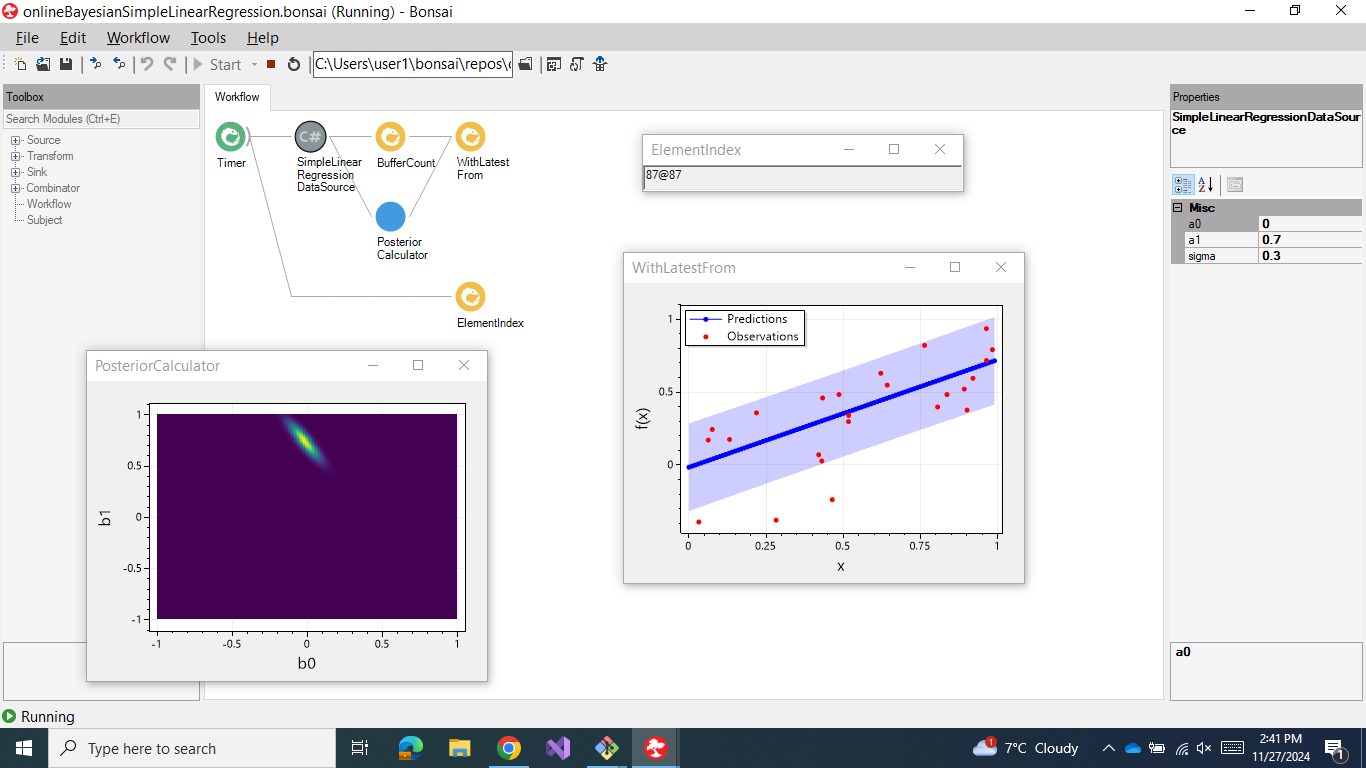
\includegraphics[width=4.0in]{figures/workflowOBLR.png}}
    \end{center}

\end{frame}

\begin{frame}
    \frametitle{Recursive least squares in Bonsai}

    \begin{center}
        \href{https://github.com/joacorapela/bonsai-rlsSimpleLinearRegression}{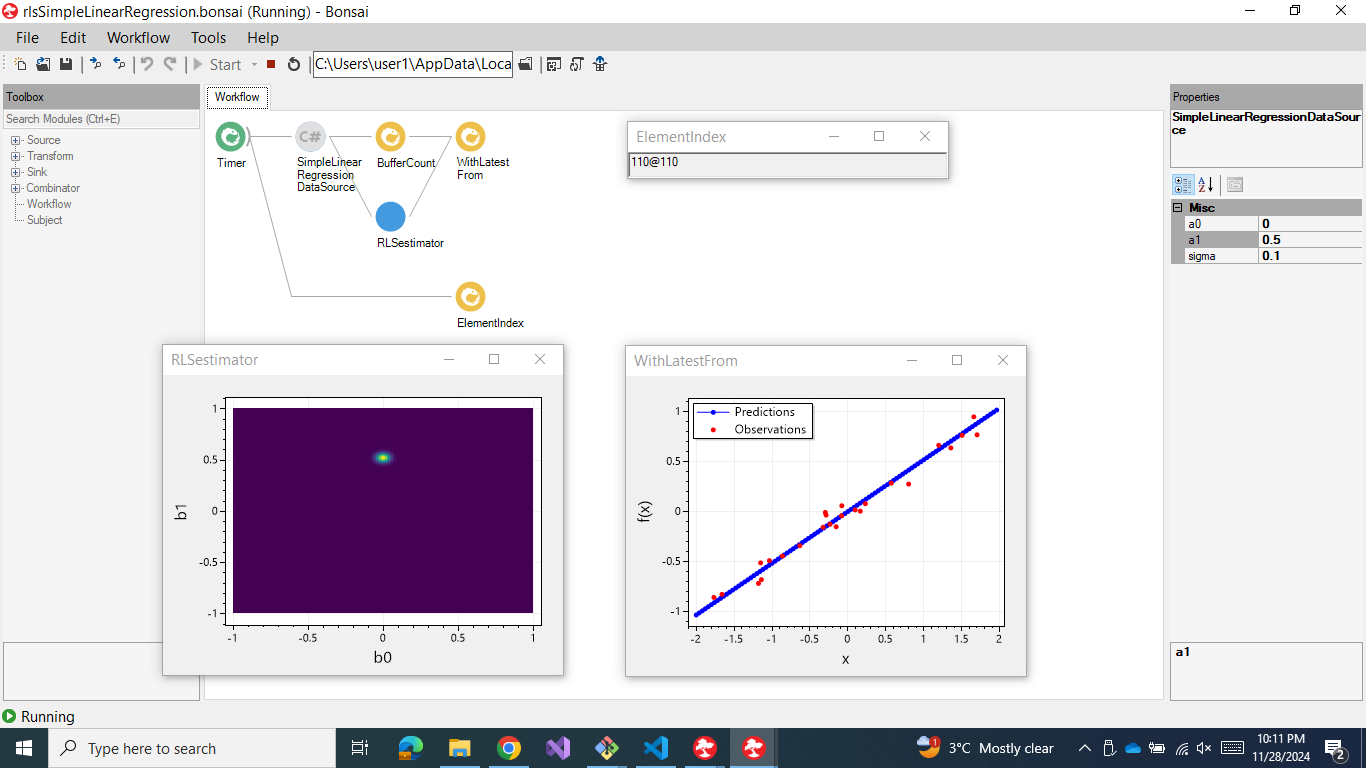
\includegraphics[width=4.0in]{figures/workflowRLS.png}}
    \end{center}

\end{frame}

\begin{frame}
    \frametitle{Estimating receptive fields of cortical visual neurons in Bonsai}

    \begin{center}
        \href{https://github.com/joacorapela/bonsai-oblr-corticalSimpleCellEx}{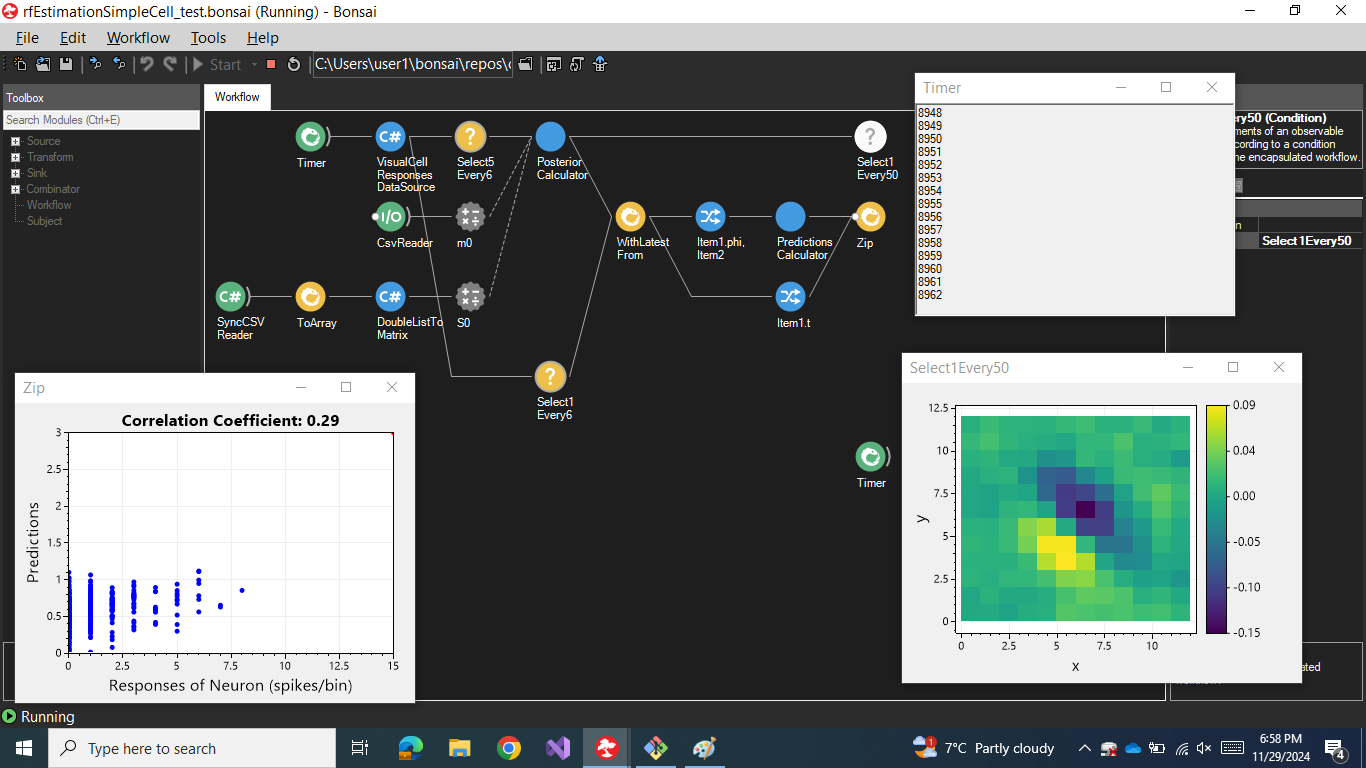
\includegraphics[width=4.0in]{figures/workflowOBLRsimpleCell.png}}
    \end{center}

\end{frame}

\begin{frame}
    \frametitle{References}

    \tiny{
        \bibliographystyle{apalike}
        \bibliography{probability,informationTheory,machineLearning,gaussianProcesses,latentsVariablesModels,linearDynamicalSystems,numericalMethods}
    }
\end{frame}

\end{document}


\section{Bonsai-Python Integration}

\begin{frame}
    \frametitle{Bonsai-Python Integration: Fundamental Concepts}

    \begin{itemize}
        \item architecture
        \item async/sync regimes
    \end{itemize}

\end{frame}

\begin{frame}
    \frametitle{Bonsai-Python Integration: Practical}

    \begin{itemize}
        \item Bonsai-Python Hello World
        \item Bonsai-Python advanced example
    \end{itemize}

\end{frame}

\section{Linear Dynamical Systems}

\begin{frame}
    \frametitle{Linear Dynamical Systems: Fundamental Concepts}

    Fundamental concepts of LDS.

\end{frame}

\begin{frame}
    \frametitle{Linear Dynamical Systems: Practical}

    Estimation of foraging mice kinematics.

\end{frame}

\section{Hidden Markov Models}

\begin{frame}
    \frametitle{Hidden Markov Models: Fundamental Concepts}

    Fundamental concepts of HMMs.

\end{frame}

\begin{frame}
    \frametitle{Hidden Markov Models: Practical}

    Estimation of behavioral states of foraging mice.

\end{frame}

\section{State-Space Decoders}

\begin{frame}
    \frametitle{State-Space Decoders: Fundamental Concepts}

    Fundamental concepts of state-space decoders.

\end{frame}

\begin{frame}
    \frametitle{State-Space Decoders: Practical}

    Mice position decoding from hippocampal population activity.

\end{frame}

\section{Discussion}

\begin{frame}
    \frametitle{Discussion}

    \begin{itemize}
        \item interactions between experimental and computational
            neuroscientists (documentation)

        \item Bonsai.ML roadmap

            \begin{itemize}

                \item our proposal
                \item suggestions?

            \end{itemize}

        \item suggestions for:

            \begin{itemize}
                \item new ML models to integrate into Bonsai
                \item new applications areas to investigate with Bonsai.ML
            \end{itemize}

    \end{itemize}

\end{frame}

\begin{frame}
    \frametitle{References}

    \tiny{
        \bibliographystyle{apalike}
        \bibliography{probability,informationTheory,machineLearning,gaussianProcesses,latentsVariablesModels,linearDynamicalSystems,numericalMethods}
    }
\end{frame}

\end{document}
